\section{第 5 章综合习题}

\begin{problem}{三角函数系的正交性}{Orthogonality-Of-Trigonometric-System}
    设 $m, n$ 为正整数，证明：
    \begin{enumerate}
        \item $\int_0^{2\uppi} \sin mx \cdot \cos nx \d x = 0$；
        \item $\int_0^{2\uppi} \sin mx \cdot \sin nx \d x = \int_0^{2\uppi} \cos mx \cdot \cos nx \d x = \begin{dcases} \uppi, & m = n, \\ 0, & m \neq n. \end{dcases}$
    \end{enumerate}
    （本题的结论，在以后要讲的傅里叶级数理论中具有基本的重要性．）
\end{problem}

\begin{myproof}
    \ansitem{1}

    利用积化和差公式 $\sin mx \cos nx = \frac{1}{2}\bigl(\sin(m+n)x + \sin(m-n)x\bigr)$：
    \begin{enumerate}
        \item 当 $m \neq n$ 时：
              \begin{equation}
                  \begin{aligned}
                      \int_0^{2\uppi} \sin mx \cos nx \d x & = \frac{1}{2} \int_0^{2\uppi} \bigl(\sin(m+n)x + \sin(m-n)x\bigr) \d x                        \\
                                                           & = \frac{1}{2} \left[ -\frac{\cos(m+n)x}{m+n} - \frac{\cos(m-n)x}{m-n} \right]_0^{2\uppi} = 0;
                  \end{aligned}
              \end{equation}
        \item 当 $m = n$ 时：
              \begin{equation}
                  \int_0^{2\uppi} \sin mx \cos mx \d x = \frac{1}{2}\int_0^{2\uppi} \sin 2mx \d x = \left[ -\frac{\cos 2mx}{4m} \right]_0^{2\uppi} = 0.
              \end{equation}
    \end{enumerate}
    综合可知，恒有 $\int_0^{2\uppi} \sin mx \cos nx \d x = 0$．

    \ansitem{2}

    利用积化和差公式分别展开：
    \begin{enumerate}
        \item 对于正弦乘积项，由 $\sin mx \sin nx = \frac{1}{2}\bigl(\cos(m-n)x - \cos(m+n)x\bigr)$：
              若 $m \neq n$，则
              \begin{equation}
                  \int_0^{2\uppi} \sin mx \sin nx \d x = \frac{1}{2} \left[ \frac{\sin(m-n)x}{m-n} - \frac{\sin(m+n)x}{m+n} \right]_0^{2\uppi} = 0;
              \end{equation}
              若 $m = n$，则
              \begin{equation}
                  \int_0^{2\uppi} \sin^2 mx \d x = \int_0^{2\uppi} \frac{1 - \cos 2mx}{2} \d x = \left[ \frac{x}{2} - \frac{\sin 2mx}{4m} \right]_0^{2\uppi} = \uppi.
              \end{equation}
        \item 对于余弦乘积项，由 $\cos mx \cos nx = \frac{1}{2}\bigl(\cos(m-n)x + \cos(m+n)x\bigr)$：
              若 $m \neq n$，则
              \begin{equation}
                  \int_0^{2\uppi} \cos mx \cos nx \d x = \frac{1}{2} \left[ \frac{\sin(m-n)x}{m-n} + \frac{\sin(m+n)x}{m+n} \right]_0^{2\uppi} = 0;
              \end{equation}
              若 $m = n$，则
              \begin{equation}
                  \int_0^{2\uppi} \cos^2 mx \d x = \int_0^{2\uppi} \frac{1 + \cos 2mx}{2} \d x = \left[ \frac{x}{2} + \frac{\sin 2mx}{4m} \right]_0^{2\uppi} = \uppi.
              \end{equation}
    \end{enumerate}
    命题得证．
\end{myproof}

\begin{problem}{Beta函数的性质与阶乘表示}{Beta-Function-Properties-And-Factorial-Representation}
    设 $m, n$ 为正整数，记
    \begin{equation}
        B(m, n) = \int_0^1 x^m (1 - x)^n \d x.
    \end{equation}
    证明：
    \begin{enumerate}
        \item $B(m, n) = B(n, m)$；
        \item $B(m, n) = \frac{m!n!}{(m+n+1)!}$．
    \end{enumerate}
    $B(m, n)$ 是著名的 Beta 函数（简称 $\text{B}$-函数）的特例．一般的 $B(m, n)$，对 $m > -1$ 及 $n > -1$ 都有意义，我们将在以后讨论．习题5.1中第6.(2)题，给出了 $m > 0, n > 0$ 时，$B(m, n)$ 的一个上界估计．
\end{problem}

\begin{myproof}
    \ansitem{1}

    作变量代换 $x = 1 - t$，则 $\d x = -\d t$，积分限由 $0 \to 1$ 变为 $1 \to 0$：
    \begin{equation}
        B(m, n) = \int_1^0 (1 - t)^m t^n (-\d t) = \int_0^1 t^n (1 - t)^m \d t = B(n, m).
    \end{equation}

    \ansitem{2}

    应用分部积分法建立递推关系：
    \begin{equation}
        \begin{aligned}
            B(m, n) & = \int_0^1 (1 - x)^n \d\left( \frac{x^{m+1}}{m+1} \right)                                            \\
                    & = \left[ \frac{x^{m+1}(1 - x)^n}{m+1} \right]_0^1 + \frac{n}{m+1} \int_0^1 x^{m+1}(1 - x)^{n-1} \d x \\
                    & = \frac{n}{m+1} B(m+1, n-1).
        \end{aligned}
    \end{equation}
    连续应用此递推关系 $n$ 次：
    \begin{equation}
        \begin{aligned}
            B(m, n) & = \frac{n}{m+1} \cdot \frac{n-1}{m+2} \cdots \frac{1}{m+n} B(m+n, 0) \\
                    & = \frac{n!}{(m+1)(m+2)\cdots(m+n)} \int_0^1 x^{m+n} \d x             \\
                    & = \frac{n!}{(m+1)(m+2)\cdots(m+n)(m+n+1)}                            \\
                    & = \frac{m!n!}{(m+n+1)!}.
        \end{aligned}
    \end{equation}
\end{myproof}

\begin{problem}{若干定积分的综合计算}{Definite-Integrals-Calculation-Collection}
    计算下列积分：
    \begin{enumerate}
        \item $\int_{\frac{1}{2}}^2 \left(1 + x - \frac{1}{x}\right) \e^{x + \frac{1}{x}} \d x$；
        \item $\int_0^{n\uppi} x |\sin x| \d x$（$n$ 为正整数）；
        \item 设 $f(x) = \int_x^{x+2\uppi}(1 + \e^{\sin t} - \e^{-\sin t})\d t + \frac{1}{1+x}\int_0^1 f(t)\d t$，求 $\int_0^1 f(x) \d x$．
    \end{enumerate}
\end{problem}

\begin{solution}
    \ansitem{1}

    注意到被积函数满足精确微分关系：
    \begin{equation}
        \frac{\d}{\d x}\left( x \e^{x + \frac{1}{x}} \right) = \e^{x + \frac{1}{x}} + x\left(1 - \frac{1}{x^2}\right)\e^{x + \frac{1}{x}} = \left(1 + x - \frac{1}{x}\right)\e^{x + \frac{1}{x}}.
    \end{equation}
    由 Newton-Leibniz 公式直接求解：
    \begin{equation}
        \int_{\frac{1}{2}}^2 \left(1 + x - \frac{1}{x}\right) \e^{x + \frac{1}{x}} \d x = \left[ x \e^{x + \frac{1}{x}} \right]_{\frac{1}{2}}^2 = 2\e^{\frac{5}{2}} - \frac{1}{2}\e^{\frac{5}{2}} = \frac{3}{2}\e^2\sqrt{\e}.
    \end{equation}
    \begin{equation}
        \boxed{\int_{\frac{1}{2}}^2 \left(1 + x - \frac{1}{x}\right) \e^{x + \frac{1}{x}} \d x = \frac{3}{2}\e^2\sqrt{\e}.}
    \end{equation}

    \ansitem{2}

    将积分区间拆分为 $n$ 个长度为 $\uppi$ 的子区间之和：
    \begin{equation}
        \int_0^{n\uppi} x |\sin x| \d x = \sum_{k=1}^n \int_{(k-1)\uppi}^{k\uppi} x |\sin x| \d x.
    \end{equation}
    在每个子区间上作变量代换 $x = t + (k-1)\uppi$（$t \in [0, \uppi]$）：
    \begin{equation}
        \begin{aligned}
            \int_{(k-1)\uppi}^{k\uppi} x |\sin x| \d x & = \int_0^{\uppi} \bigl(t + (k-1)\uppi\bigr)\sin t \d t                 \\
                                                       & = \int_0^{\uppi} t \sin t \d t + (k-1)\uppi \int_0^{\uppi} \sin t \d t \\
                                                       & = \uppi + 2(k-1)\uppi = (2k - 1)\uppi.
        \end{aligned}
    \end{equation}
    对所有子区间求和：
    \begin{equation}
        \int_0^{n\uppi} x |\sin x| \d x = \sum_{k=1}^n (2k - 1)\uppi = n^2 \uppi.
    \end{equation}
    \begin{equation}
        \boxed{\int_0^{n\uppi} x |\sin x| \d x = n^2 \uppi.}
    \end{equation}

    \ansitem{3}

    记常数 $A = \int_0^1 f(t)\d t$．

    由于被积函数 $g(t) = 1 + \e^{\sin t} - \e^{-\sin t}$ 是以 $2\uppi$ 为周期的连续函数，其在任意长度为 $2\uppi$ 的区间上的积分均相等：
    \begin{equation}
        \int_x^{x+2\uppi} \bigl(1 + \e^{\sin t} - \e^{-\sin t}\bigr)\d t = \int_0^{2\uppi} 1 \d t + \int_0^{2\uppi} \bigl(\e^{\sin t} - \e^{-\sin t}\bigr)\d t = 2\uppi + 0 = 2\uppi.
    \end{equation}
    因此 $f(x) = 2\uppi + \frac{A}{1 + x}$．在区间 $[0, 1]$ 上积分：
    \begin{equation}
        A = \int_0^1 \left( 2\uppi + \frac{A}{1 + x} \right) \d x = 2\uppi + A [\ln(1 + x)]_0^1 = 2\uppi + A\ln 2.
    \end{equation}
    解得 $A(1 - \ln 2) = 2\uppi \implies A = \frac{2\uppi}{1 - \ln 2}$．
    \begin{equation}
        \boxed{\int_0^1 f(x) \d x = \frac{2\uppi}{1 - \ln 2}.}
    \end{equation}
\end{solution}

\begin{problem}{正切函数高次幂积分的不等式估计}{Tangent-Power-Integral-Inequality-Estimation}
    证明：$\frac{1}{2n+2} < \int_0^{\frac{\uppi}{4}} \tan^n x \d x < \frac{1}{2n}$（$n = 1, 2, \dots$）．
\end{problem}

\begin{myproof}
    记 $I_n = \int_0^{\frac{\uppi}{4}} \tan^n x \d x$．

    利用三角恒等式 $1 + \tan^2 x = \sec^2 x$ 计算递推关系：
    \begin{equation}
        I_n + I_{n+2} = \int_0^{\frac{\uppi}{4}} \tan^n x (1 + \tan^2 x)\d x = \int_0^{\frac{\uppi}{4}} \tan^n x \d(\tan x) = \left[ \frac{\tan^{n+1} x}{n+1} \right]_0^{\frac{\uppi}{4}} = \frac{1}{n+1}.
    \end{equation}
    当 $x \in \left(0, \frac{\uppi}{4}\right)$ 时，恒有 $0 < \tan x < 1$，故序列 $\{I_n\}$ 严格单调递减：
    \begin{equation}
        I_{n+2} < I_{n+1} < I_n < I_{n-1}.
    \end{equation}
    由 $I_{n+2} < I_n$，得
    \begin{equation}
        2I_n > I_n + I_{n+2} = \frac{1}{n+1} \implies I_n > \frac{1}{2n+2}.
    \end{equation}
    另一方面，对任意 $n \geqslant 1$，有
    \begin{equation}
        I_{n-1} + I_{n+1} - 2I_n = \int_0^{\frac{\uppi}{4}} \tan^{n-1} x (1 - \tan x)^2 \d x > 0.
    \end{equation}
    从而
    \begin{equation}
        2I_n < I_{n-1} + I_{n+1} = \frac{1}{n} \implies I_n < \frac{1}{2n}.
    \end{equation}
    综合两式，即证
    \begin{equation}
        \frac{1}{2n+2} < \int_0^{\frac{\uppi}{4}} \tan^n x \d x < \frac{1}{2n}.
    \end{equation}
\end{myproof}

\begin{problem}{可积函数积分正性的区间局部性质}{Integrable-Function-Positive-Integral-Local-Property}
    设函数 $f$ 在 $[a, b]$ 上可积，且 $\int_a^b f(x) \d x > 0$，证明：必有一个区间 $[\alpha, \beta] \subset [a, b]$，使得对任意 $x \in [\alpha, \beta]$，有 $f(x) > 0$．（比较习题5.1中第8题：设 $f$ 是区间 $[a, b]$ 上的连续函数．若 $\int_a^b f(x) \d x = 0$，则 $f$ 在 $(a, b)$ 中至少有一个零点．因此，由函数的积分这一整体信息，能够推断函数值的某些性质．）

    （提示：假设结论不对，则对 $[a, b]$ 的任一划分 $a = x_0 < x_1 < \cdots < x_{n-1} < x_n = b$，在区间 $[x_{i-1}, x_i]$ 上都存在 $\xi_i$，使 $f(\xi_i) \leqslant 0$．由此产生一个非正的积分和，过渡到极限，产生矛盾．）
\end{problem}

\begin{myproof}
    采用反证法．

    假设结论不成立，即在 $[a, b]$ 的任意子区间 $[\alpha, \beta]$ 上，均存在点 $x$ 满足 $f(x) \leqslant 0$．

    任取区间 $[a, b]$ 的一个分割 $T : a = x_0 < x_1 < \cdots < x_n = b$．由假设，在每个子区间 $[x_{i-1}, x_i]$（$i = 1, 2, \dots, n$）上必存在一点 $\xi_i \in [x_{i-1}, x_i]$，使得
    \begin{equation}
        f(\xi_i) \leqslant 0.
    \end{equation}
    构造对应的 Riemann 和：
    \begin{equation}
        \sigma(f, T, \{\xi_i\}) = \sum_{i=1}^n f(\xi_i)\Delta x_i \leqslant 0.
    \end{equation}
    因为函数 $f$ 在 $[a, b]$ 上 Riemann 可积，根据定积分的定义，当分割细度 $\|T\| = \max_{1\leqslant i\leqslant n} \Delta x_i \to 0$ 时，Riemann 和的极限与介点选取无关且等于定积分：
    \begin{equation}
        \int_a^b f(x)\d x = \lim_{\|T\|\to 0} \sum_{i=1}^n f(\xi_i)\Delta x_i \leqslant 0.
    \end{equation}
    这与已知条件 $\int_a^b f(x)\d x > 0$ 产生矛盾．

    因此假设不成立，必存在区间 $[\alpha, \beta] \subset [a, b]$，使得对任意 $x \in [\alpha, \beta]$，均有 $f(x) > 0$．
\end{myproof}

\begin{problem}{连续奇偶函数的原函数对称性}{Antiderivatives-Symmetry-Of-Even-And-Odd-Functions}
    \begin{enumerate}
        \item 设 $f$ 是处处连续的偶函数，则 $f$ 必有一个原函数为奇函数；
        \item 设 $f$ 是处处连续的奇函数，则 $f$ 的任一个原函数都是偶函数．
    \end{enumerate}
    （试比较习题3.1第15题：证明：可导的偶函数的导数为奇函数；而可导的奇函数的导数为偶函数．）
\end{problem}

\begin{myproof}
    \ansitem{1}

    定义变上限积分函数
    \begin{equation}
        F(x) = \int_0^x f(t) \d t.
    \end{equation}
    由于 $f$ 处处连续，由微积分基本定理可知 $F'(x) = f(x)$，即 $F(x)$ 为 $f(x)$ 的一个原函数．

    对任意 $x \in \symbb{R}$，作变量代换 $t = -u$：
    \begin{equation}
        F(-x) = \int_0^{-x} f(t) \d t = \int_0^x f(-u)(-\d u) = -\int_0^x f(u) \d u = -F(x).
    \end{equation}
    因此 $F(x)$ 是奇函数，即 $f$ 必有一个原函数为奇函数．

    \ansitem{2}

    设 $G(x)$ 为 $f$ 在 $\symbb{R}$ 上的任意一个原函数．由原函数族性质，存在常数 $C$ 使得
    \begin{equation}
        G(x) = \int_0^x f(t) \d t + C.
    \end{equation}
    对任意 $x \in \symbb{R}$，作变量代换 $t = -u$ 并利用 $f$ 为奇函数的性质 $f(-u) = -f(u)$：
    \begin{equation}
        \int_0^{-x} f(t) \d t = \int_0^x f(-u)(-\d u) = \int_0^x \bigl(-f(u)\bigr)(-\d u) = \int_0^x f(u) \d u.
    \end{equation}
    因此
    \begin{equation}
        G(-x) = \int_0^{-x} f(t) \d t + C = \int_0^x f(t) \d t + C = G(x).
    \end{equation}
    这表明 $G(x)$ 为偶函数，即 $f$ 的任一个原函数都是偶函数．
\end{myproof}

\begin{problem}{连续周期函数的非周期原函数}{Continuous-Periodic-Function-Nonperiodic-Antiderivative}
    举例说明，存在一个连续的周期函数 $f$，使得 $f$ 的原函数都不是周期函数．（提示：选一个连续的周期函数 $f$，使它能保证 $F(x) = \int_0^x f(t) \d t$ 不是周期函数．注意，不必考虑 $F(x)$ 的显式表示．）
\end{problem}

\begin{solution}
    取常数函数 $f(x) = 1$（或 $f(x) = 1 + \sin x$）．

    显然 $f(x)$ 在 $\symbb{R}$ 上连续，且是以任何 $T > 0$（对 $1 + \sin x$ 则以 $T = 2\uppi$）为周期的周期函数．

    $f(x)$ 的任意原函数均可表示为
    \begin{equation}
        F(x) = \int_0^x 1 \d t + C = x + C \quad (C \in \symbb{R}).
    \end{equation}
    由于
    \begin{equation}
        \lim_{x\to +\infty} F(x) = \lim_{x\to +\infty} (x + C) = +\infty,
    \end{equation}
    $F(x)$ 为无界函数（且严格单调递增）．而任何定义在 $\symbb{R}$ 上的连续周期函数必然是有界的，故 $F(x)$ 绝不可能是周期函数．

    因此，$f(x)$ 的所有原函数都不是周期函数．
    \begin{equation}
        \boxed{f(x) = 1 \text{（或 } f(x) = 1 + \sin x\text{）为满足条件的连续周期函数．}}
    \end{equation}
\end{solution}

\begin{problem}{多项式零点存在性的积分证明}{Polynomial-Root-Existence-Via-Integration}
    设 $\frac{a_0}{n+1} + \frac{a_1}{n} + \dots + a_n = 0$．证明：多项式 $a_0 x^n + a_1 x^{n-1} + \dots + a_n$ 在 $(0, 1)$ 内至少有一个零点．
\end{problem}

\begin{myproof}
    令多项式函数为
    \begin{equation}
        P(x) = a_0 x^n + a_1 x^{n-1} + \dots + a_n.
    \end{equation}
    由于 $P(x)$ 为多项式，其在闭区间 $[0, 1]$ 上连续．

    计算 $P(x)$ 在 $[0, 1]$ 上的定积分：
    \begin{equation}
        \begin{aligned}
            \int_0^1 P(x) \d x & = \int_0^1 (a_0 x^n + a_1 x^{n-1} + \dots + a_n) \d x                          \\
                               & = \left[ \frac{a_0}{n+1}x^{n+1} + \frac{a_1}{n}x^n + \dots + a_n x \right]_0^1 \\
                               & = \frac{a_0}{n+1} + \frac{a_1}{n} + \dots + a_n = 0.
        \end{aligned}
    \end{equation}
    由积分第一中值定理，由于 $P(x)$ 在 $[0, 1]$ 上连续，必存在 $\xi \in (0, 1)$，使得
    \begin{equation}
        \int_0^1 P(x) \d x = P(\xi)(1 - 0) = P(\xi).
    \end{equation}
    结合积分值为零的条件，即有
    \begin{equation}
        P(\xi) = 0.
    \end{equation}
    故多项式 $P(x)$ 在开区间 $(0, 1)$ 内至少存在一个零点 $\xi$．
\end{myproof}

\begin{problem}{三角加权积分为零的函数零点个数}{Trigonometric-Weighted-Integral-Zeros}
    设函数 $f$ 在 $[0, \uppi]$ 上连续，且有 $\int_0^{\uppi} f(x) \sin x \d x = \int_0^{\uppi} f(x) \cos x \d x = 0$．试证：在 $(0, \uppi)$ 内存在两点 $x_1$ 和 $x_2$，使得 $f(x_1) = f(x_2) = 0$．

    （提示：易知 $f$ 在 $(0, \uppi)$ 内至少有一个零点 $x_1$．若这是唯一的零点，则 $f$ 在 $(0, x_1)$ 与 $(x_1, \uppi)$ 内异号．于是 $\int_0^{\uppi} f(x)\sin(x - x_1)\d x \neq 0$，这将产生矛盾．）
\end{problem}

\begin{myproof}
    第一步，证明 $f(x)$ 在 $(0, \uppi)$ 内至少有一个零点且变号．

    若 $f(x)$ 在 $(0, \uppi)$ 内不变号（不妨设 $f(x) \geqslant 0$ 且 $f(x) \not\equiv 0$），由于当 $x \in (0, \uppi)$ 时 $\sin x > 0$，故乘积 $f(x)\sin x \geqslant 0$ 且不恒为零．由连续非负函数积分的正性，有
    \begin{equation}
        \int_0^{\uppi} f(x) \sin x \d x > 0,
    \end{equation}
    这与已知条件 $\int_0^{\uppi} f(x) \sin x \d x = 0$ 矛盾．因此，$f(x)$ 在 $(0, \uppi)$ 内至少存在一个变号零点，记为 $x_1 \in (0, \uppi)$．

    第二步，采用反证法证明 $f(x)$ 在 $(0, \uppi)$ 内至少存在两个零点．

    假设 $f(x)$ 在 $(0, \uppi)$ 内不存在除 $x_1$ 之外的其他变号零点，则 $f(x)$ 在区间 $(0, x_1)$ 与 $(x_1, \uppi)$ 上分别保持恒定符号，且符号相反．

    考察辅助函数 $\sin(x - x_1)$：
    \begin{equation}
        \sin(x - x_1) \begin{dcases} < 0, & x \in (0, x_1), \\ > 0, & x \in (x_1, \uppi). \end{dcases}
    \end{equation}
    因此，函数乘积 $f(x)\sin(x - x_1)$ 在两个子区间 $(0, x_1)$ 与 $(x_1, \uppi)$ 上均同号（恒同为正或恒同为负），且在 $(0, \uppi)$ 上不恒为零．

    由定积分性质，其在 $[0, \uppi]$ 上的积分必不为零：
    \begin{equation}
        \int_0^{\uppi} f(x) \sin(x - x_1) \d x \neq 0.
    \end{equation}
    另一方面，利用正弦和差角公式展开积分：
    \begin{equation}
        \begin{aligned}
            \int_0^{\uppi} f(x) \sin(x - x_1) \d x & = \int_0^{\uppi} f(x) (\sin x \cos x_1 - \cos x \sin x_1) \d x                        \\
                                                   & = \cos x_1 \int_0^{\uppi} f(x) \sin x \d x - \sin x_1 \int_0^{\uppi} f(x) \cos x \d x \\
                                                   & = \cos x_1 \cdot 0 - \sin x_1 \cdot 0 = 0.
        \end{aligned}
    \end{equation}
    两式相矛盾，故假设不成立．

    因此，$f(x)$ 在 $(0, \uppi)$ 内至少存在两个相异的零点 $x_1$ 和 $x_2$，即 $f(x_1) = f(x_2) = 0$．
\end{myproof}

\begin{problem}{含参变限积分的可微性与导数计算}{Differentiability-Of-Parameter-Integral}
    设 $f(x)$ 处处连续，$f(0) = 0$，且 $f'(0)$ 存在．记 $F(x) = \int_0^1 f(xy) \d y$．证明：$F(x)$ 处处可导，并求出 $F'(x)$．
\end{problem}

\begin{solution}
    当 $x \neq 0$ 时，作变量代换 $u = xy$，则 $\d y = \frac{\d u}{x}$，积分变为
    \begin{equation}
        F(x) = \frac{1}{x}\int_0^x f(u) \d u.
    \end{equation}
    当 $x = 0$ 时，$F(0) = \int_0^1 f(0) \d y = \int_0^1 0 \d y = 0$．

    讨论导数的存在性与求导运算：
    \begin{enumerate}
        \item 当 $x \neq 0$ 时，因为 $f(u)$ 处处连续，由微积分基本定理可知变上限积分 $\int_0^x f(u)\d u$ 可导且导数为 $f(x)$．由商的求导法则，$F(x)$ 必可导，且
              \begin{equation}
                  F'(x) = \frac{\d}{\d x}\left( \frac{1}{x}\int_0^x f(u)\d u \right) = \frac{x f(x) - \int_0^x f(u)\d u}{x^2} = \frac{f(x) - F(x)}{x};
              \end{equation}
        \item 当 $x = 0$ 时，根据导数定义考察差商的极限：
              \begin{equation}
                  F'(0) = \lim_{x\to 0} \frac{F(x) - F(0)}{x - 0} = \lim_{x\to 0} \frac{\frac{1}{x}\int_0^x f(u)\d u}{x} = \lim_{x\to 0} \frac{\int_0^x f(u)\d u}{x^2}.
              \end{equation}
              由于 $\lim_{x\to 0} \int_0^x f(u)\d u = 0$，分母 $\lim_{x\to 0} x^2 = 0$，应用 L'Hôpital 法则并利用导数定义：
              \begin{equation}
                  F'(0) = \lim_{x\to 0} \frac{f(x)}{2x} = \frac{1}{2} \lim_{x\to 0} \frac{f(x) - f(0)}{x - 0} = \frac{1}{2} f'(0).
              \end{equation}
    \end{enumerate}
    综合可知，$F(x)$ 在 $\symbb{R}$ 上处处可导．
    \begin{equation}
        \boxed{F'(x) = \begin{dcases} \frac{x f(x) - \int_0^x f(u)\d u}{x^2}, & x \neq 0, \\ \frac{1}{2}f'(0), & x = 0. \end{dcases}}
    \end{equation}
\end{solution}

\begin{problem}{变上限积分的可微性与单侧导数}{Upper-Limit-Integral-Differentiability-And-One-Sided-Derivative}
    \begin{enumerate}
        \item 设 $f(x) = \begin{dcases} \e^{-x^2}, & |x| \leqslant 1, \\ 1, & |x| > 1. \end{dcases}$ 记 $F(x) = \int_0^x f(t) \d t$．试研究 $F(x)$ 在哪些点可导．

              （提示：与习题5.1第16题不同，本题无法求出 $F(x)$ 的显式表示．）
        \item 设 $f(x) = \int_0^x \cos \frac{1}{t} \d t$，求证 $f'_+(0) = 0$．
    \end{enumerate}
\end{problem}

\begin{solution}
    \ansitem{1}

    考察被积函数 $f(t)$ 的连续性：
    $f(t)$ 在 $(-\infty, -1)$、$(-1, 1)$ 及 $(1, +\infty)$ 上均连续，而在 $t = \pm 1$ 处有
    \begin{equation}
        \lim_{t\to 1^-} f(t) = \e^{-1}, \qquad \lim_{t\to 1^+} f(t) = 1,
    \end{equation}
    \begin{equation}
        \lim_{t\to -1^+} f(t) = \e^{-1}, \qquad \lim_{t\to -1^-} f(t) = 1.
    \end{equation}
    故 $t = \pm 1$ 为 $f(t)$ 的第一类跳跃间断点．

    对于变上限积分 $F(x) = \int_0^x f(t) \d t$：
    \begin{enumerate}
        \item 当 $x \neq \pm 1$ 时，$f(t)$ 在 $t = x$ 处连续，由微积分基本定理，$F'(x) = f(x)$ 存在；
        \item 当 $x = 1$ 时，分别计算左、右单侧导数：
              \begin{equation}
                  F'_+(1) = \lim_{h\to 0^+} \frac{1}{h}\int_1^{1+h} f(t)\d t = \lim_{h\to 0^+} \frac{1}{h}\int_1^{1+h} 1 \d t = 1,
              \end{equation}
              \begin{equation}
                  F'_-(1) = \lim_{h\to 0^+} \frac{1}{-h}\int_1^{1-h} f(t)\d t = \lim_{h\to 0^+} \frac{1}{h}\int_{1-h}^1 \e^{-t^2} \d t = \e^{-1}.
              \end{equation}
              因为 $F'_+(1) \neq F'_-(1)$，所以 $F(x)$ 在 $x = 1$ 处不可导；
        \item 同理，在 $x = -1$ 处，计算单侧导数：
              \begin{equation}
                  F'_+(-1) = \e^{-1}, \qquad F'_-(-1) = 1.
              \end{equation}
              因为 $F'_+(-1) \neq F'_-(-1)$，所以 $F(x)$ 在 $x = -1$ 处不可导．
    \end{enumerate}
    因此，$F(x)$ 在集合 $\symbb{R} \setminus \{-1, 1\}$ 上处处可导．
    \begin{equation}
        \boxed{F(x) \text{ 在 } x \in (-\infty, -1) \cup (-1, 1) \cup (1, +\infty) \text{ 上可导．}}
    \end{equation}

    \ansitem{2}

    根据右导数的定义，需证
    \begin{equation}
        f'_+(0) = \lim_{x\to 0^+} \frac{f(x) - f(0)}{x - 0} = \lim_{x\to 0^+} \frac{1}{x} \int_0^x \cos \frac{1}{t} \d t = 0.
    \end{equation}
    对任意 $x > 0$，利用恒等式 $\cos\frac{1}{t}\d t = -t^2 \d\left(\sin\frac{1}{t}\right)$，对反常积分应用分部积分法：
    \begin{equation}
        \begin{aligned}
            \int_0^x \cos \frac{1}{t} \d t & = \lim_{\varepsilon\to 0^+} \int_\varepsilon^x \cos \frac{1}{t} \d t                                                                      \\
                                           & = \lim_{\varepsilon\to 0^+} \left( \left[ -t^2 \sin\frac{1}{t} \right]_\varepsilon^x + \int_\varepsilon^x 2t \sin\frac{1}{t} \d t \right) \\
                                           & = -x^2 \sin\frac{1}{x} + \int_0^x 2t \sin\frac{1}{t} \d t.
        \end{aligned}
    \end{equation}
    两端同除以 $x$：
    \begin{equation}
        \frac{1}{x}\int_0^x \cos \frac{1}{t} \d t = -x \sin\frac{1}{x} + \frac{1}{x} \int_0^x 2t \sin\frac{1}{t} \d t.
    \end{equation}
    分别进行绝对值放大估计：
    \begin{equation}
        \left| -x \sin\frac{1}{x} \right| \leqslant x \xrightarrow{x\to 0^+} 0,
    \end{equation}
    \begin{equation}
        \left| \frac{1}{x}\int_0^x 2t \sin\frac{1}{t} \d t \right| \leqslant \frac{1}{x} \int_0^x 2t \left|\sin\frac{1}{t}\right| \d t \leqslant \frac{1}{x} \int_0^x 2t \d t = \frac{x^2}{x} = x \xrightarrow{x\to 0^+} 0.
    \end{equation}
    由夹逼准则，两项极限均为 $0$，故
    \begin{equation}
        f'_+(0) = \lim_{x\to 0^+} \frac{1}{x}\int_0^x \cos\frac{1}{t}\d t = 0.
    \end{equation}
\end{solution}

\begin{problem}{连续函数差商积分极限的证明}{Limit-Of-Difference-Quotient-Integral}
    设函数 $f$ 处处连续．证明：
    \begin{equation}
        \lim_{h\to 0} \frac{1}{h}\int_a^b \bigl(f(x + h) - f(x)\bigr) \d x = f(b) - f(a).
    \end{equation}
    （提醒：本题容易做错．）
\end{problem}

\begin{myproof}
    定义变上限积分函数
    \begin{equation}
        F(u) = \int_a^u f(t) \d t.
    \end{equation}
    因为 $f$ 在 $\symbb{R}$ 上处处连续，由微积分基本定理，$F(u)$ 在 $\symbb{R}$ 上处处可导，且对任意 $u \in \symbb{R}$ 恒有 $F'(u) = f(u)$．

    将定积分拆项并对第一项作平移换元 $u = x + h$：
    \begin{equation}
        \int_a^b f(x + h) \d x = \int_{a+h}^{b+h} f(u) \d u = \int_a^{b+h} f(u)\d u - \int_a^{a+h} f(u)\d u = F(b + h) - F(a + h).
    \end{equation}
    而第二项积分为
    \begin{equation}
        \int_a^b f(x) \d x = F(b) - F(a).
    \end{equation}
    因此，被求极限的差商表达式可精确化简为
    \begin{equation}
        \begin{aligned}
            \frac{1}{h}\int_a^b \bigl(f(x + h) - f(x)\bigr) \d x & = \frac{\bigl(F(b + h) - F(a + h)\bigr) - \bigl(F(b) - F(a)\bigr)}{h} \\
                                                                 & = \frac{F(b + h) - F(b)}{h} - \frac{F(a + h) - F(a)}{h}.
        \end{aligned}
    \end{equation}
    两端取 $h \to 0$ 的极限，根据导数的定义：
    \begin{equation}
        \begin{aligned}
            \lim_{h\to 0} \frac{1}{h}\int_a^b \bigl(f(x + h) - f(x)\bigr) \d x & = \lim_{h\to 0}\frac{F(b + h) - F(b)}{h} - \lim_{h\to 0}\frac{F(a + h) - F(a)}{h} \\
                                                                               & = F'(b) - F'(a)                                                                   \\
                                                                               & = f(b) - f(a).
        \end{aligned}
    \end{equation}
    命题得证．
\end{myproof}

\begin{problem}{黎曼-勒贝格引理的证明}{Riemann-Lebesgue-Lemma}
    设函数 $f(x)$ 在 $[a, b]$ 上连续可微．证明：
    \begin{equation}
        \lim_{\lambda\to \infty} \int_a^b f(x) \sin \lambda x \d x = 0.
    \end{equation}
    （提示：分部积分．）
\end{problem}

\begin{myproof}
    应用分部积分法，将被积表达式进行变形：
    \begin{equation}
        \begin{aligned}
            \int_a^b f(x) \sin \lambda x \d x & = \int_a^b f(x) \d\left( -\frac{\cos \lambda x}{\lambda} \right)                                                  \\
                                              & = \left[ -\frac{f(x)\cos \lambda x}{\lambda} \right]_a^b + \frac{1}{\lambda} \int_a^b f'(x) \cos \lambda x \d x   \\
                                              & = \frac{f(a)\cos \lambda a - f(b)\cos \lambda b}{\lambda} + \frac{1}{\lambda} \int_a^b f'(x) \cos \lambda x \d x.
        \end{aligned}
    \end{equation}
    因为 $f(x)$ 在闭区间 $[a, b]$ 上连续可微，所以导函数 $f'(x)$ 在 $[a, b]$ 上连续，从而在 $[a, b]$ 上有界，即存在常数 $M > 0$，使得对任意 $x \in [a, b]$ 均有 $|f'(x)| \leqslant M$．

    对各项分别进行绝对值放大估计：
    \begin{equation}
        \left| \frac{f(a)\cos \lambda a - f(b)\cos \lambda b}{\lambda} \right| \leqslant \frac{|f(a)| + |f(b)|}{|\lambda|},
    \end{equation}
    \begin{equation}
        \left| \frac{1}{\lambda} \int_a^b f'(x) \cos \lambda x \d x \right| \leqslant \frac{1}{|\lambda|} \int_a^b |f'(x)| \d x \leqslant \frac{M(b - a)}{|\lambda|}.
    \end{equation}
    由三角不等式，有
    \begin{equation}
        \left| \int_a^b f(x) \sin \lambda x \d x \right| \leqslant \frac{|f(a)| + |f(b)| + M(b - a)}{|\lambda|}.
    \end{equation}
    当 $\lambda \to \infty$ 时，上式右端趋于 $0$．由夹逼准则，即得
    \begin{equation}
        \lim_{\lambda\to \infty} \int_a^b f(x) \sin \lambda x \d x = 0.
    \end{equation}
    命题得证．
\end{myproof}

\begin{problem}{正弦绝对值积分的均值极限}{Limit-Of-Periodic-Integral-Mean}
    证明：
    \begin{equation}
        \lim_{x\to +\infty} \frac{1}{x} \int_0^x |\sin t| \d t = \frac{2}{\uppi}.
    \end{equation}
\end{problem}

\begin{myproof}
    函数 $|\sin t|$ 为以 $\uppi$ 为周期的连续函数，其在单个周期上的积分值为
    \begin{equation}
        \int_0^{\uppi} |\sin t| \d t = \int_0^{\uppi} \sin t \d t = [-\cos t]_0^{\uppi} = 2.
    \end{equation}
    对任意 $x > 0$，设 $x = n\uppi + r$，其中 $n = \lfloor \frac{x}{\uppi} \rfloor \in \symbb{N}$ 为整数部分，$r \in [0, \uppi)$ 为余项．

    将积分区间拆分为周期部分与余项部分：
    \begin{equation}
        \int_0^x |\sin t| \d t = \sum_{k=1}^n \int_{(k-1)\uppi}^{k\uppi} |\sin t| \d t + \int_{n\uppi}^{n\uppi + r} |\sin t| \d t = 2n + \int_0^r \sin t \d t.
    \end{equation}
    由于被积函数非负，余项积分满足界估计：
    \begin{equation}
        0 \leqslant \int_0^r \sin t \d t \leqslant \int_0^{\uppi} \sin t \d t = 2.
    \end{equation}
    因此恒有
    \begin{equation}
        2n \leqslant \int_0^x |\sin t| \d t \leqslant 2n + 2.
    \end{equation}
    两端同除以 $x = n\uppi + r$：
    \begin{equation}
        \frac{2n}{n\uppi + r} \leqslant \frac{1}{x}\int_0^x |\sin t| \d t \leqslant \frac{2n + 2}{n\uppi + r}.
    \end{equation}
    当 $x \to +\infty$ 时，必有 $n \to \infty$．分别考察两端的极限：
    \begin{equation}
        \lim_{n\to \infty} \frac{2n}{n\uppi + r} = \lim_{n\to \infty} \frac{2}{\uppi + \frac{r}{n}} = \frac{2}{\uppi},
    \end{equation}
    \begin{equation}
        \lim_{n\to \infty} \frac{2n + 2}{n\uppi + r} = \lim_{n\to \infty} \frac{2 + \frac{2}{n}}{\uppi + \frac{r}{n}} = \frac{2}{\uppi}.
    \end{equation}
    由夹逼准则，即得
    \begin{equation}
        \lim_{x\to +\infty} \frac{1}{x}\int_0^x |\sin t| \d t = \frac{2}{\uppi}.
    \end{equation}
\end{myproof}

\begin{problem}{正弦高次幂积分的极限}{Limit-Of-Sine-Power-Integral}
    证明：$\lim_{n\to \infty} \int_0^{\frac{\uppi}{2}} \sin^n x \d x = 0$．

    （提示：直接用积分中值定理，得出所说的积分为 $\frac{\uppi}{2} \sin^n \xi_n$（其中 $0 < \xi_n < \frac{\uppi}{2}$），但这不能导出结果，因不能排除 $\{\xi_n\}$ 中有一个子列趋于 $\frac{\uppi}{2}$．克服这一困难可采用如下的方法．对任意正数 $\varepsilon < 1$，取一个参数 $\delta$（与 $\varepsilon$ 有关），将问题中的积分拆成两部分：一部分用区间长度控制；另一部分由 $n \to \infty$ 来控制，以使得两者的和小于 $\varepsilon$．我们有
    \begin{equation}
        \int_0^{\frac{\uppi}{2}} \sin^n x \d x = \int_0^{\frac{\uppi}{2} - \delta} \sin^n x \d x + \int_{\frac{\uppi}{2} - \delta}^{\frac{\uppi}{2}} \sin^n x \d x < 2\left[ \sin\left(\frac{\uppi}{2} - \delta\right) \right]^n + \delta = 2\cos^n \delta + \delta.
    \end{equation}
    现在取 $\delta = \frac{\varepsilon}{2}$，因 $0 < \cos\frac{\varepsilon}{2} < 1$，且 $\cos\frac{\varepsilon}{2}$ 与 $n$ 无关，故 $n$ 充分大时，可使上式第一项小于 $\frac{\varepsilon}{2}$．
    解答本题的另一方法是应用 \S5.1 中例9．参考第 1 章综合习题中第 1 题中的 (1)．）
\end{problem}

\begin{solution}
    解法一（区间拆分与 $\varepsilon$-$\delta$ 估计法）：

    对任意给定的 $\varepsilon \in (0, 1)$，取 $\delta = \frac{\varepsilon}{2} \in \left(0, \frac{\uppi}{4}\right)$．将积分区间拆分为 $\left[0, \frac{\uppi}{2} - \delta\right]$ 与 $\left[\frac{\uppi}{2} - \delta, \frac{\uppi}{2}\right]$ 两部分：
    \begin{equation}
        \int_0^{\frac{\uppi}{2}} \sin^n x \d x = \int_0^{\frac{\uppi}{2} - \delta} \sin^n x \d x + \int_{\frac{\uppi}{2} - \delta}^{\frac{\uppi}{2}} \sin^n x \d x.
    \end{equation}
    对于第一项，因为 $\sin x$ 在区间 $\left[0, \frac{\uppi}{2} - \delta\right]$ 上单调递增，其最大值为 $\sin\left(\frac{\uppi}{2} - \delta\right) = \cos\delta$，所以
    \begin{equation}
        \int_0^{\frac{\uppi}{2} - \delta} \sin^n x \d x \leqslant \left(\frac{\uppi}{2} - \delta\right)\cos^n \delta < \frac{\uppi}{2}\cos^n \delta < 2\cos^n \delta.
    \end{equation}
    对于第二项，利用被积函数 $\sin^n x \leqslant 1$ 控制积分值：
    \begin{equation}
        \int_{\frac{\uppi}{2} - \delta}^{\frac{\uppi}{2}} \sin^n x \d x \leqslant 1 \cdot \left( \frac{\uppi}{2} - \left(\frac{\uppi}{2} - \delta\right) \right) = \delta = \frac{\varepsilon}{2}.
    \end{equation}
    将两部分相加，得到
    \begin{equation}
        0 < \int_0^{\frac{\uppi}{2}} \sin^n x \d x < 2\cos^n\left(\frac{\varepsilon}{2}\right) + \frac{\varepsilon}{2}.
    \end{equation}
    由于 $0 < \frac{\varepsilon}{2} < \frac{\uppi}{4}$，故 $0 < \cos\left(\frac{\varepsilon}{2}\right) < 1$ 且与 $n$ 无关，从而
    \begin{equation}
        \lim_{n\to \infty} 2\cos^n\left(\frac{\varepsilon}{2}\right) = 0.
    \end{equation}
    因此存在正整数 $N$，使得当 $n > N$ 时恒有 $2\cos^n\left(\frac{\varepsilon}{2}\right) < \frac{\varepsilon}{2}$．于是对所有 $n > N$，均有
    \begin{equation}
        0 < \int_0^{\frac{\uppi}{2}} \sin^n x \d x < \frac{\varepsilon}{2} + \frac{\varepsilon}{2} = \varepsilon.
    \end{equation}
    由数列极限的定义，即证 $\lim_{n\to \infty} \int_0^{\frac{\uppi}{2}} \sin^n x \d x = 0$．

    解法二（Wallis 递推关系与夹逼准则）：

    记 $I_n = \int_0^{\frac{\uppi}{2}} \sin^n x \d x$．由分部积分法可知数列满足递推公式：
    \begin{equation}
        I_n = \frac{n-1}{n} I_{n-2} \quad (n \geqslant 2).
    \end{equation}
    从而有
    \begin{equation}
        n I_n I_{n-1} = (n-1) I_{n-1} I_{n-2} = \dots = 1 \cdot I_1 I_0 = 1 \cdot 1 \cdot \frac{\uppi}{2} = \frac{\uppi}{2}.
    \end{equation}
    因此对任意 $n \geqslant 1$，恒有
    \begin{equation}
        I_n I_{n-1} = \frac{\uppi}{2n}.
    \end{equation}
    当 $x \in \left(0, \frac{\uppi}{2}\right)$ 时，恒有 $0 < \sin x < 1$，故序列 $\{I_n\}$ 严格单调递减：
    \begin{equation}
        0 < I_n < I_{n-1}.
    \end{equation}
    两端同乘 $I_n$ 得
    \begin{equation}
        0 < I_n^2 < I_n I_{n-1} = \frac{\uppi}{2n} \implies 0 < I_n < \sqrt{\frac{\uppi}{2n}}.
    \end{equation}
    当 $n \to \infty$ 时，$\lim_{n\to \infty} \sqrt{\frac{\uppi}{2n}} = 0$．由夹逼准则，即得
    \begin{equation}
        \lim_{n\to \infty} \int_0^{\frac{\uppi}{2}} \sin^n x \d x = 0.
    \end{equation}
    \begin{equation}
        \boxed{\lim_{n\to \infty} \int_0^{\frac{\uppi}{2}} \sin^n x \d x = 0.}
    \end{equation}
\end{solution}

\begin{problem}{非负连续函数的积分范数极限}{Lp-Norm-Limit-Of-Continuous-Function}
    设 $f(x)$ 是 $[a, b]$ 上的连续函数，且 $f(x) \geqslant 0$（对 $x \in [a, b]$）．记 $f(x)$ 在这区间上的最大值为 $M$，证明：
    \begin{equation}
        \lim_{n\to \infty} \left( \int_a^b f^n(x) \d x \right)^{\frac{1}{n}} = M.
    \end{equation}
\end{problem}

\begin{myproof}
    若 $M = 0$，由 $f(x) \geqslant 0$ 可知 $f(x) \equiv 0$，此时结论显然成立．下设 $M > 0$．

    一方面，由最大值定义，对任意 $x \in [a, b]$ 均有 $0 \leqslant f(x) \leqslant M$．由定积分的保序性：
    \begin{equation}
        \int_a^b f^n(x) \d x \leqslant \int_a^b M^n \d x = M^n (b - a).
    \end{equation}
    两端开 $n$ 次方：
    \begin{equation}
        \left( \int_a^b f^n(x) \d x \right)^{\frac{1}{n}} \leqslant M (b - a)^{\frac{1}{n}}.
    \end{equation}
    两端取上极限：
    \begin{equation}
        \limsup_{n\to \infty} \left( \int_a^b f^n(x) \d x \right)^{\frac{1}{n}} \leqslant \lim_{n\to \infty} M (b - a)^{\frac{1}{n}} = M.
    \end{equation}
    另一方面，对任意给定的 $\varepsilon \in (0, M)$，根据连续函数的闭区间最大值定理，存在 $x_0 \in [a, b]$ 使得 $f(x_0) = M > M - \varepsilon$．

    由连续函数的保号性，存在子区间 $[\alpha, \beta] \subset [a, b]$（满足 $\beta - \alpha > 0$），使得对任意 $x \in [\alpha, \beta]$ 均有
    \begin{equation}
        f(x) \geqslant M - \varepsilon.
    \end{equation}
    由被积函数的非负性，缩小子区间积分范围：
    \begin{equation}
        \int_a^b f^n(x) \d x \geqslant \int_\alpha^\beta f^n(x) \d x \geqslant \int_\alpha^\beta (M - \varepsilon)^n \d x = (M - \varepsilon)^n (\beta - \alpha).
    \end{equation}
    两端开 $n$ 次方：
    \begin{equation}
        \left( \int_a^b f^n(x) \d x \right)^{\frac{1}{n}} \geqslant (M - \varepsilon)(\beta - \alpha)^{\frac{1}{n}}.
    \end{equation}
    两端取下极限：
    \begin{equation}
        \liminf_{n\to \infty} \left( \int_a^b f^n(x) \d x \right)^{\frac{1}{n}} \geqslant \lim_{n\to \infty} (M - \varepsilon)(\beta - \alpha)^{\frac{1}{n}} = M - \varepsilon.
    \end{equation}
    由 $\varepsilon > 0$ 的任意性，令 $\varepsilon \to 0^+$ 可得
    \begin{equation}
        \liminf_{n\to \infty} \left( \int_a^b f^n(x) \d x \right)^{\frac{1}{n}} \geqslant M.
    \end{equation}
    结合上极限与下极限的不等式：
    \begin{equation}
        M \leqslant \liminf_{n\to \infty} \left( \int_a^b f^n(x) \d x \right)^{\frac{1}{n}} \leqslant \limsup_{n\to \infty} \left( \int_a^b f^n(x) \d x \right)^{\frac{1}{n}} \leqslant M.
    \end{equation}
    因此极限存在且等于 $M$：
    \begin{equation}
        \lim_{n\to \infty} \left( \int_a^b f^n(x) \d x \right)^{\frac{1}{n}} = M.
    \end{equation}
    命题得证．
\end{myproof}

\begin{problem}{单调函数求和与积分的差值估计与极限}{Monotone-Function-Sum-Integral-Inequalities}
    \begin{enumerate}
        \item 设 $f(x)$ 是 $[1, +\infty)$ 上的递增、非负函数，证明：对任意正整数 $n$，有
              \begin{equation}
                  0 \leqslant \sum_{k=1}^n f(k) - \int_1^n f(x) \d x \leqslant f(n);
              \end{equation}
        \item 设 $f(x)$ 是 $[1, +\infty)$ 上的递减、非负函数，证明：对任意正整数 $n$，有
              \begin{equation}
                  0 \leqslant \sum_{k=1}^n f(k) - \int_1^n f(x) \d x \leqslant f(1).
              \end{equation}
              此外，极限
              \begin{equation}
                  \lim_{n\to\infty} \left( \sum_{k=1}^n f(k) - \int_1^n f(x) \d x \right) = \alpha
              \end{equation}
              存在，且 $0 \leqslant \alpha \leqslant f(1)$．
    \end{enumerate}
    （提示：对于 (1)，应用习题 5.1中第 5 题可知，
    \begin{equation}
        f(k) \leqslant \int_k^{k+1} f(x) \d x \leqslant f(k+1),
    \end{equation}
    对 $k = 1, 2, \dots, n-1$ 求和，可得出结果．类似地可证明 (2) 中的不等式．
    为证明 (2) 中说的极限存在，可证明
    \begin{equation}
        g(n) = \sum_{k=1}^n f(k) - \int_1^n f(x) \d x, \quad n = 1, 2, \dots
    \end{equation}
    是单调递减的函数；而上面已指出 $g(n)$ 以 $0$ 为下界．）

    某些（不易直接处理的）离散的量——数列的和，可以通过（易于处理的）连续的量——积分作出估计，本题给出了最简单的这样的结果（这在后面的无穷级数理论中还将提及）．例如，我们现在易于给出 $\sum_{k=1}^n \sqrt{k}$ 及 $n!$ 的相当精确的上、下界．我们特别提及，对 $n \geqslant 1$，有
    \begin{equation}
        \ln n \leqslant \sum_{k=1}^n \frac{1}{k} \leqslant \ln n + 1,
    \end{equation}
    从而 $\sum_{k=1}^n \frac{1}{k}$ 趋于无穷大，并且与 $\ln n$ 同阶．此外，
    \begin{equation}
        \gamma = \lim_{n\to\infty} \left( \sum_{k=1}^n \frac{1}{k} - \ln n \right)
    \end{equation}
    存在，这称为 Euler 常数．
\end{problem}

\begin{solution}
    \ansitem{1}

    因为 $f(x)$ 在 $[1, +\infty)$ 上单调递增，所以在每个子区间 $[k, k+1]$（$k = 1, 2, \dots, n-1$）上，对任意 $x \in [k, k+1]$ 恒有
    \begin{equation}
        f(k) \leqslant f(x) \leqslant f(k+1).
    \end{equation}
    由定积分的保序性，在区间 $[k, k+1]$ 上积分得
    \begin{equation}
        f(k) \leqslant \int_k^{k+1} f(x) \d x \leqslant f(k+1).
    \end{equation}
    将上述不等式对 $k = 1, 2, \dots, n-1$ 逐项累加求和：
    \begin{equation}
        \sum_{k=1}^{n-1} f(k) \leqslant \sum_{k=1}^{n-1} \int_k^{k+1} f(x) \d x \leqslant \sum_{k=1}^{n-1} f(k+1).
    \end{equation}
    由定积分的可加性，中间项为 $\int_1^n f(x) \d x$．改写求和指标可得
    \begin{equation}
        \sum_{k=1}^n f(k) - f(n) \leqslant \int_1^n f(x) \d x \leqslant \sum_{k=1}^n f(k) - f(1).
    \end{equation}
    分别进行移项：
    \begin{enumerate}
        \item 由右边不等式 $\int_1^n f(x) \d x \leqslant \sum_{k=1}^n f(k) - f(1)$ 及 $f(1) \geqslant 0$，得
              \begin{equation}
                  \sum_{k=1}^n f(k) - \int_1^n f(x) \d x \geqslant f(1) \geqslant 0;
              \end{equation}
        \item 由左边不等式 $\sum_{k=1}^n f(k) - f(n) \leqslant \int_1^n f(x) \d x$，得
              \begin{equation}
                  \sum_{k=1}^n f(k) - \int_1^n f(x) \d x \leqslant f(n).
              \end{equation}
    \end{enumerate}
    综合即证
    \begin{equation}
        0 \leqslant \sum_{k=1}^n f(k) - \int_1^n f(x) \d x \leqslant f(n).
    \end{equation}

    \ansitem{2}

    第一步，建立不等式估计．

    因为 $f(x)$ 在 $[1, +\infty)$ 上单调递减，所以在每个子区间 $[k, k+1]$（$k = 1, 2, \dots, n-1$）上，对任意 $x \in [k, k+1]$ 恒有
    \begin{equation}
        f(k+1) \leqslant f(x) \leqslant f(k).
    \end{equation}
    在区间 $[k, k+1]$ 上积分：
    \begin{equation}
        f(k+1) \leqslant \int_k^{k+1} f(x) \d x \leqslant f(k).
    \end{equation}
    对 $k = 1, 2, \dots, n-1$ 求和：
    \begin{equation}
        \sum_{k=1}^{n-1} f(k+1) \leqslant \sum_{k=1}^{n-1} \int_k^{k+1} f(x) \d x \leqslant \sum_{k=1}^{n-1} f(k),
    \end{equation}
    即
    \begin{equation}
        \sum_{k=1}^n f(k) - f(1) \leqslant \int_1^n f(x) \d x \leqslant \sum_{k=1}^n f(k) - f(n).
    \end{equation}
    分别移项并利用 $f(n) \geqslant 0$：
    \begin{enumerate}
        \item 由左端不等式得
              \begin{equation}
                  \sum_{k=1}^n f(k) - \int_1^n f(x) \d x \leqslant f(1);
              \end{equation}
        \item 由右端不等式得
              \begin{equation}
                  \sum_{k=1}^n f(k) - \int_1^n f(x) \d x \geqslant f(n) \geqslant 0.
              \end{equation}
    \end{enumerate}
    从而对任意正整数 $n$，恒有
    \begin{equation}
        0 \leqslant \sum_{k=1}^n f(k) - \int_1^n f(x) \d x \leqslant f(1).
    \end{equation}

    \begin{center}
        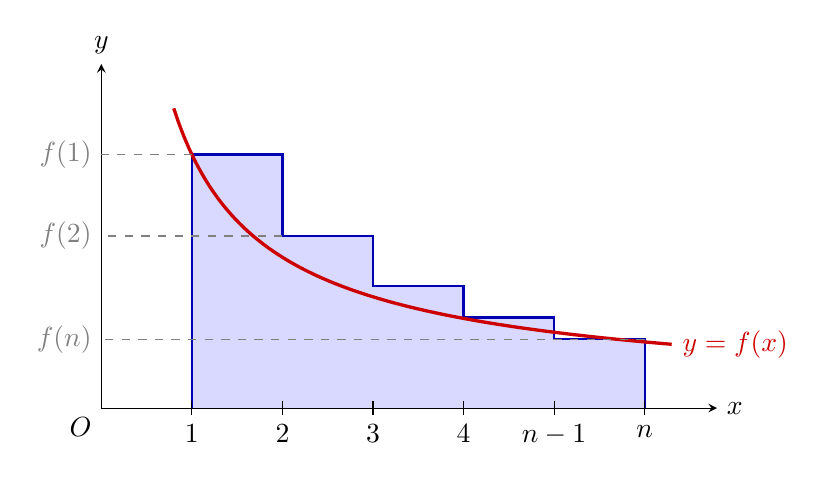
\begin{tikzpicture}[>=stealth, scale=1.15]
            \draw[->] (0, 0) -- (6.8, 0) node[right] {$x$};
            \draw[->] (0, 0) -- (0, 3.8) node[above] {$y$};
            \node[below left] at (0, 0) {$O$};

            % Rectangles corresponding to sum_{k=1}^n f(k)
            \fill[blue!15] (1, 0) rectangle (2, 2.8);
            \fill[blue!15] (2, 0) rectangle (3, 1.9);
            \fill[blue!15] (3, 0) rectangle (4, 1.35);
            \fill[blue!15] (4, 0) rectangle (5, 1.0);
            \fill[blue!15] (5, 0) rectangle (6, 0.76);

            \draw[blue!70!black, thick] (1, 0) -- (1, 2.8) -- (2, 2.8) -- (2, 1.9) -- (3, 1.9)
            -- (3, 1.35) -- (4, 1.35) -- (4, 1.0) -- (5, 1.0) -- (5, 0.76) -- (6, 0.76) -- (6, 0);

            % Curve y = f(x)
            \draw[domain=0.8:6.3, samples=100, smooth, very thick, red!80!black]
            plot (\x, {2.8 / (\x^0.75)}) node[right] {$y = f(x)$};

            \draw[dashed, gray] (1, 2.8) -- (0, 2.8) node[left] {$f(1)$};
            \draw[dashed, gray] (2, 1.9) -- (0, 1.9) node[left] {$f(2)$};
            \draw[dashed, gray] (6, 0.76) -- (0, 0.76) node[left] {$f(n)$};

            \foreach \x/\xtext in {1/1, 2/2, 3/3, 4/4, 5/n-1, 6/n} {
                    \draw (\x, 0.08) -- (\x, -0.08) node[below] {$\xtext$};
                }
        \end{tikzpicture}
    \end{center}

    第二步，证明极限的存在性．

    记数列
    \begin{equation}
        g(n) = \sum_{k=1}^n f(k) - \int_1^n f(x) \d x \quad (n = 1, 2, \dots).
    \end{equation}
    计算相邻项的差值：
    \begin{equation}
        \begin{aligned}
            g(n+1) - g(n) & = \left( \sum_{k=1}^{n+1} f(k) - \int_1^{n+1} f(x) \d x \right) - \left( \sum_{k=1}^n f(k) - \int_1^n f(x) \d x \right) \\
                          & = f(n+1) - \int_n^{n+1} f(x) \d x.
        \end{aligned}
    \end{equation}
    因为 $f(x)$ 递减，当 $x \in [n, n+1]$ 时恒有 $f(x) \geqslant f(n+1)$，故
    \begin{equation}
        \int_n^{n+1} f(x) \d x \geqslant \int_n^{n+1} f(n+1) \d x = f(n+1).
    \end{equation}
    由此可得
    \begin{equation}
        g(n+1) - g(n) = f(n+1) - \int_n^{n+1} f(x) \d x \leqslant 0.
    \end{equation}
    因此数列 $\{g(n)\}$ 单调递减．

    又由第一步已证的不等式可知，对任意 $n \geqslant 1$ 恒有 $g(n) \geqslant 0$，即 $\{g(n)\}$ 有下界 $0$．

    根据单调有界收敛准则，极限 $\lim_{n\to\infty} g(n)$ 必存在，记为 $\alpha$．

    由于 $0 \leqslant g(n) \leqslant f(1)$ 对任意 $n \geqslant 1$ 成立，由极限的保序性可得
    \begin{equation}
        0 \leqslant \alpha \leqslant f(1).
    \end{equation}

    \begin{equation}
        \boxed{\lim_{n\to\infty} \left( \sum_{k=1}^n f(k) - \int_1^n f(x) \d x \right) = \alpha \quad (0 \leqslant \alpha \leqslant f(1)).}
    \end{equation}
\end{solution}

\begin{problem}{Cauchy 积分不等式及其取等条件}{Cauchy-Schwarz-Integral-Inequality}
    (Cauchy 积分不等式) 设 $f(x)$ 与 $g(x)$ 在 $[a, b]$ 上连续，证明：
    \begin{equation}
        \left(\int_a^b f(x)g(x)\d x\right)^2 \leqslant \int_a^b f^2(x)\d x \int_a^b g^2(x)\d x,
    \end{equation}
    等号成立的充分必要条件是：$f$ 和 $g$ 中有一个恒为零，或 $f(x) = \lambda g(x)$（对 $x \in [a, b]$），这里 $\lambda$ 是一个常数．

    （提示：本题有好几种证法．用积分上限求导可得出一个证明，参见习题5.1中第 28 题的提示．最标准的方法如下：不妨设 $\int_a^b g^2(x)\d x \neq 0$，否则易知函数 $g$ 恒为零，结论显然成立（习题5.1 第 4(2) 题）．考虑关于 $t$ 的二次三项式 $\int_a^b (f(x) + tg(x))^2 \d x$，这总是非负的．）
\end{problem}

\begin{myproof}
    第一步，证明不等式成立．

    若 $\int_a^b g^2(x)\d x = 0$，由 $g(x)$ 在 $[a, b]$ 上的连续性与非负性可知 $g(x) \equiv 0$，此时不等式两端均为 $0$，不等式显然成立．

    若 $\int_a^b g^2(x)\d x > 0$，对任意实数 $t \in \symbb{R}$，考察非负连续函数 $(f(x) + tg(x))^2 \geqslant 0$ 的定积分：
    \begin{equation}
        P(t) = \int_a^b (f(x) + tg(x))^2 \d x = t^2 \int_a^b g^2(x)\d x + 2t \int_a^b f(x)g(x)\d x + \int_a^b f^2(x)\d x \geqslant 0.
    \end{equation}
    $P(t)$ 是关于 $t$ 的实系数一元二次三项式，其二次项系数满足 $\int_a^b g^2(x)\d x > 0$．

    因为对任意 $t \in \symbb{R}$ 恒有 $P(t) \geqslant 0$，故判别式必满足 $\Delta \leqslant 0$：
    \begin{equation}
        \Delta = 4\left(\int_a^b f(x)g(x)\d x\right)^2 - 4\left(\int_a^b g^2(x)\d x\right)\left(\int_a^b f^2(x)\d x\right) \leqslant 0,
    \end{equation}
    即
    \begin{equation}
        \left(\int_a^b f(x)g(x)\d x\right)^2 \leqslant \int_a^b f^2(x)\d x \int_a^b g^2(x)\d x.
    \end{equation}

    第二步，证明等号成立的充要条件．
    \begin{enumerate}
        \item 充分性：若 $g(x) \equiv 0$ 或 $f(x) \equiv 0$，两端均为 $0$，等号成立；若存在常数 $\lambda$ 使得 $f(x) = \lambda g(x)$，则
              \begin{equation}
                  \left(\int_a^b f(x)g(x)\d x\right)^2 = \left(\int_a^b \lambda g^2(x)\d x\right)^2 = \lambda^2 \left(\int_a^b g^2(x)\d x\right)^2,
              \end{equation}
              \begin{equation}
                  \int_a^b f^2(x)\d x \int_a^b g^2(x)\d x = \left(\int_a^b \lambda^2 g^2(x)\d x\right)\left(\int_a^b g^2(x)\d x\right) = \lambda^2 \left(\int_a^b g^2(x)\d x\right)^2,
              \end{equation}
              两端相等，等号成立．
        \item 必要性：若等号成立且 $g(x) \not\equiv 0$，则 $\Delta = 0$，二次方程 $P(t) = 0$ 存在唯一实根 $t_0$：
              \begin{equation}
                  t_0 = -\frac{\int_a^b f(x)g(x)\d x}{\int_a^b g^2(x)\d x}.
              \end{equation}
              此时
              \begin{equation}
                  P(t_0) = \int_a^b (f(x) + t_0 g(x))^2 \d x = 0.
              \end{equation}
              由于 $(f(x) + t_0 g(x))^2$ 在 $[a, b]$ 上连续且非负，其积分为零蕴含着对任意 $x \in [a, b]$ 恒有
              \begin{equation}
                  (f(x) + t_0 g(x))^2 = 0 \implies f(x) + t_0 g(x) = 0 \implies f(x) = -t_0 g(x).
              \end{equation}
              取常数 $\lambda = -t_0$，即有 $f(x) = \lambda g(x)$．
    \end{enumerate}
    命题得证．
\end{myproof}

\begin{problem}{导数连续函数的点值与积分不等式}{Function-Value-And-Integral-Inequality}
    设 $f(x)$ 在 $[0, 1]$ 上有连续的导数，证明：对任意 $a \in [0, 1]$，有
    \begin{equation}
        |f(a)| \leqslant \int_0^1 |f(x)| \d x + \int_0^1 |f'(x)| \d x.
    \end{equation}
\end{problem}

\begin{myproof}
    对任意 $x \in [0, 1]$ 与 $a \in [0, 1]$，由 Newton-Leibniz 公式可得
    \begin{equation}
        f(a) = f(x) + \int_x^a f'(t)\d t.
    \end{equation}
    两端取绝对值并利用三角不等式与定积分性质：
    \begin{equation}
        |f(a)| \leqslant |f(x)| + \left| \int_x^a f'(t)\d t \right| \leqslant |f(x)| + \int_0^1 |f'(t)|\d t.
    \end{equation}
    对上式两端关于变量 $x$ 在区间 $[0, 1]$ 上积分：
    \begin{equation}
        \int_0^1 |f(a)| \d x \leqslant \int_0^1 |f(x)| \d x + \int_0^1 \left( \int_0^1 |f'(t)|\d t \right) \d x.
    \end{equation}
    由于 $|f(a)|$ 及 $\int_0^1 |f'(t)|\d t$ 均关于变量 $x$ 为常数，积分化简为
    \begin{equation}
        |f(a)| \leqslant \int_0^1 |f(x)| \d x + \int_0^1 |f'(x)| \d x.
    \end{equation}
    命题得证．
\end{myproof}

\begin{problem}{正弦积分的不等式估计}{Sine-Integral-Inequality-Estimation}
    证明：$0.944 < \int_0^1 \frac{\sin x}{x} \d x < 0.947$．（提示：参看习题5.1中第 24 题的提示．）
\end{problem}

\begin{myproof}
    根据 $\sin x$ 的带 Lagrange 余项的 Taylor 展开式，当 $x \in (0, 1]$ 时，由于交错级数的逐项截断性质，恒有
    \begin{equation}
        x - \frac{x^3}{6} < \sin x < x - \frac{x^3}{6} + \frac{x^5}{120}.
    \end{equation}
    两端同除以 $x > 0$：
    \begin{equation}
        1 - \frac{x^2}{6} < \frac{\sin x}{x} < 1 - \frac{x^2}{6} + \frac{x^4}{120}.
    \end{equation}
    在区间 $[0, 1]$ 上逐项积分：
    \begin{enumerate}
        \item 下界估计：
              \begin{equation}
                  \int_0^1 \frac{\sin x}{x}\d x > \int_0^1 \left(1 - \frac{x^2}{6}\right)\d x = \left[ x - \frac{x^3}{18} \right]_0^1 = 1 - \frac{1}{18} = \frac{17}{18} \approx 0.9444 > 0.944;
              \end{equation}
        \item 上界估计：
              \begin{equation}
                  \begin{aligned}
                      \int_0^1 \frac{\sin x}{x}\d x & < \int_0^1 \left(1 - \frac{x^2}{6} + \frac{x^4}{120}\right)\d x                                                                          \\
                                                    & = \left[ x - \frac{x^3}{18} + \frac{x^5}{600} \right]_0^1 = 1 - \frac{1}{18} + \frac{1}{600} = \frac{1703}{1800} \approx 0.9461 < 0.947.
                  \end{aligned}
              \end{equation}
    \end{enumerate}
    综合可知
    \begin{equation}
        0.944 < \int_0^1 \frac{\sin x}{x} \d x < 0.947.
    \end{equation}
    命题得证．
\end{myproof}

\begin{problem}{连续可微函数的积分与黎曼和误差估计}{Riemann-Sum-Error-Estimation}
    设 $f(x)$ 在区间 $[0, 1]$ 上连续可微，且 $|f'(x)| \leqslant M$．证明：对任意正整数 $n$，
    \begin{equation}
        \left| \int_0^1 f(x) \d x - \frac{1}{n}\sum_{k=1}^n f\left(\frac{k}{n}\right) \right| \leqslant \frac{M}{2n}.
    \end{equation}
\end{problem}

\begin{myproof}
    将区间 $[0, 1]$ 等分为 $n$ 个子区间 $\left[\frac{k-1}{n}, \frac{k}{n}\right]$（$k = 1, 2, \dots, n$），积分差值可表示为
    \begin{equation}
        \int_0^1 f(x) \d x - \frac{1}{n}\sum_{k=1}^n f\left(\frac{k}{n}\right) = \sum_{k=1}^n \int_{\frac{k-1}{n}}^{\frac{k}{n}} \left( f(x) - f\left(\frac{k}{n}\right) \right) \d x.
    \end{equation}
    对任意 $x \in \left[\frac{k-1}{n}, \frac{k}{n}\right]$，由 Lagrange 中值定理，存在 $\xi_k \in \left(x, \frac{k}{n}\right)$ 使得
    \begin{equation}
        \left| f(x) - f\left(\frac{k}{n}\right) \right| = |f'(\xi_k)| \left( \frac{k}{n} - x \right) \leqslant M \left( \frac{k}{n} - x \right).
    \end{equation}
    利用三角不等式放大：
    \begin{equation}
        \begin{aligned}
            \left| \int_0^1 f(x) \d x - \frac{1}{n}\sum_{k=1}^n f\left(\frac{k}{n}\right) \right| & \leqslant \sum_{k=1}^n \int_{\frac{k-1}{n}}^{\frac{k}{n}} \left| f(x) - f\left(\frac{k}{n}\right) \right| \d x \\
                                                                                                  & \leqslant M \sum_{k=1}^n \int_{\frac{k-1}{n}}^{\frac{k}{n}} \left( \frac{k}{n} - x \right) \d x.
        \end{aligned}
    \end{equation}
    计算每个子区间上的积分：
    \begin{equation}
        \int_{\frac{k-1}{n}}^{\frac{k}{n}} \left( \frac{k}{n} - x \right) \d x = \left[ -\frac{1}{2}\left(\frac{k}{n} - x\right)^2 \right]_{\frac{k-1}{n}}^{\frac{k}{n}} = \frac{1}{2}\left(\frac{1}{n}\right)^2 = \frac{1}{2n^2}.
    \end{equation}
    代入求和：
    \begin{equation}
        \left| \int_0^1 f(x) \d x - \frac{1}{n}\sum_{k=1}^n f\left(\frac{k}{n}\right) \right| \leqslant M \sum_{k=1}^n \frac{1}{2n^2} = M \cdot n \cdot \frac{1}{2n^2} = \frac{M}{2n}.
    \end{equation}
    命题得证．
\end{myproof}

\begin{problem}{导数Lipschitz函数的导数平方不等式}{Lipschitz-Derivative-Function-Inequality}
    设 $f : \symbb{R} \to (0, +\infty)$ 是一个可微函数，且对任意实数 $x, y$ 满足
    \begin{equation}
        |f'(x) - f'(y)| \leqslant |x - y|.
    \end{equation}
    求证：对任意实数 $x$，有
    \begin{equation}
        (f'(x))^2 < 2f(x).
    \end{equation}
\end{problem}

\begin{myproof}
    任取 $x \in \symbb{R}$，分情况讨论 $f'(x)$ 的取值：
    \begin{enumerate}
        \item 若 $f'(x) = 0$，因为 $f(x) > 0$，所以 $(f'(x))^2 = 0 < 2f(x)$ 显然成立．
        \item 若 $f'(x) > 0$，由已知 Lipschitz 条件，对任意 $y < x$ 恒有
              \begin{equation}
                  f'(y) \geqslant f'(x) - |x - y| = f'(x) + y - x.
              \end{equation}
              令 $x_0 = x - f'(x) < x$．当 $y \in [x_0, x]$ 时，有 $f'(y) \geqslant f'(x) + y - x \geqslant 0$．

              在区间 $[x_0, x]$ 上积分：
              \begin{equation}
                  f(x) - f(x_0) = \int_{x_0}^x f'(y)\d y \geqslant \int_{x_0}^x (f'(x) + y - x)\d y.
              \end{equation}
              作换元 $u = x - y \in [0, f'(x)]$：
              \begin{equation}
                  \int_{x_0}^x (f'(x) + y - x)\d y = \int_0^{f'(x)} (f'(x) - u)\d u = \left[ f'(x)u - \frac{u^2}{2} \right]_0^{f'(x)} = \frac{(f'(x))^2}{2}.
              \end{equation}
              因此
              \begin{equation}
                  f(x) \geqslant f(x_0) + \frac{(f'(x))^2}{2}.
              \end{equation}
              因为 $f(x_0) > 0$，所以
              \begin{equation}
                  f(x) > \frac{(f'(x))^2}{2} \iff (f'(x))^2 < 2f(x).
              \end{equation}
        \item 若 $f'(x) < 0$，对任意 $y > x$ 恒有
              \begin{equation}
                  f'(y) \leqslant f'(x) + (y - x).
              \end{equation}
              令 $x_0 = x - f'(x) = x + |f'(x)| > x$．当 $y \in [x, x_0]$ 时，有 $f'(y) \leqslant f'(x) + y - x \leqslant 0$．

              在区间 $[x, x_0]$ 上积分：
              \begin{equation}
                  f(x) - f(x_0) = -\int_x^{x_0} f'(y)\d y \geqslant \int_x^{x_0} (-f'(x) - (y - x))\d y.
              \end{equation}
              作换元 $u = y - x \in [0, -f'(x)]$：
              \begin{equation}
                  \int_x^{x_0} (-f'(x) - (y - x))\d y = \int_0^{-f'(x)} (-f'(x) - u)\d u = \frac{(-f'(x))^2}{2} = \frac{(f'(x))^2}{2}.
              \end{equation}
              因此
              \begin{equation}
                  f(x) \geqslant f(x_0) + \frac{(f'(x))^2}{2} > \frac{(f'(x))^2}{2} \iff (f'(x))^2 < 2f(x).
              \end{equation}
    \end{enumerate}
    综合上述情况，对任意实数 $x \in \symbb{R}$，恒有 $(f'(x))^2 < 2f(x)$．命题得证．
\end{myproof}

\endinput
